\section{Modules Overview}

\subsection{Core Modules}
\begin{frame}{Core Modules}
    \begin{description}[<+(1)->]
        \item[ubus] Sofware communication bus which provides communication between various daemons and applications in OpenWrt~\cite{openwrt-ubus}~\cite{lutfi-ubus}~\cite{lutfi-ubox_ubus}~\cite{openwrt-rpc_guide}~\cite{openwrt-rpc_techref}.
        \item[ubox] General purpose library which provides features like an event loop, binary blob message formatting and handling, linked list, and some JSON helpers~\cite{openwrt-ubox}~\cite{openwrt-libubox}~\cite{lutfi-ubox_ubus}~\cite{openwrt-log}.
        \item[uci] Configuration interface aimed to centralize the configuration of OpenWrt~\cite{openwrt-uci}~\cite{openwrt-libuci}.
        \item[procd] Process manager~\cite{openwrt-procd}.
        \item[opkg] Package manager~\cite{openwrt-opkg}.
    \end{description}
\end{frame}

\subsection{Logical Structure}
\begin{frame}{Logical Structure}
    \centerline{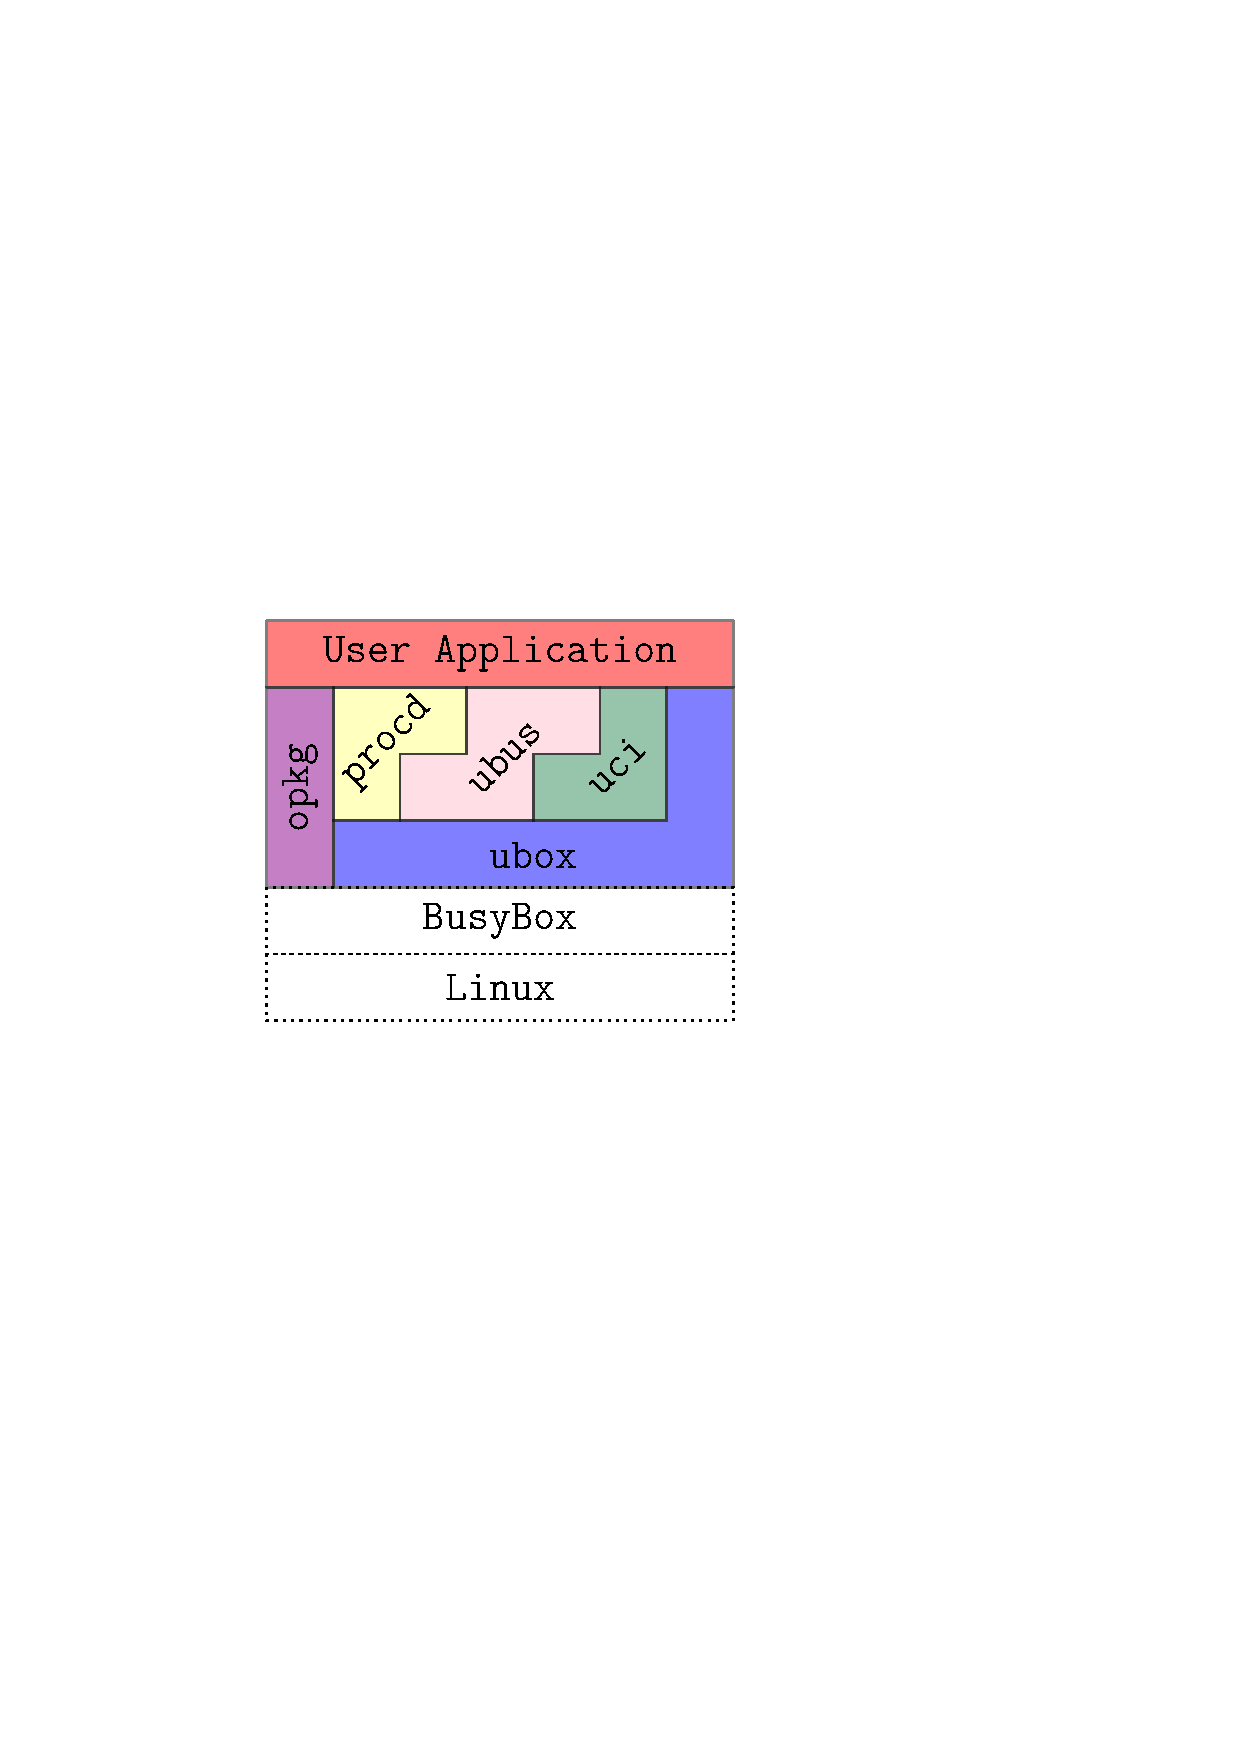
\includegraphics[width=\textheight,keepaspectratio]{openwrt-modules}}
\end{frame}
